\documentclass{stdlocal}
\begin{document}
\section{Preliminaries} % (fold)
\label{sec:preliminaries}

To systematically approach the design and implementation of curve smoothing algorithms for surface meshes, basic knowledge in the topic of differential geometry of curves and its application and generalization to polyhedral surfaces and surface mesh curves is administrable.
It allows to rigorously formulate the initial and boundary value problems for discrete geodesics which build the foundation of curve smoothing as geodesics can be interpreted as the class of smoothest curves.
Alas, differential geometry heavily builds on the mathematical tools given in the topic of analysis on manifolds and, as a consequence, the reader is assumed to be familiar with its basic concepts.
For convenience, section~\ref{sec:analysis_on_manifolds} in the appendix still provides a brief introduction to the topic to remind of and clarify notations.
% In the following, a brief overview of the main concepts is given.

\subsection{Differential Geometry of Curves} % (fold)
\label{sub:differential_geometry}

  The theory of smooth curves in space or smooth surfaces is one of the main concerns of classical differential geometry.
  Therefore, we refer to some standard textbooks, namely \textcite{goldhorn2009}, \textcite{carmo2016}, \textcite{kuehnel2013}, and \textcite{stahl2013}, for a more excessive and thorough introduction on this topic.
  For the purpose of consistent notation and as a reminder, the main concepts of smooth curves are briefly given in the following in the sense of classical and modern differential geometry based on these books.

  In the fields of analysis and numerical mathematics, it is a natural approach to extend a well-founded and -understood theory for smooth objects to their discrete counterparts and vice versa.
  Hereby, discrete or smooth objects will be typically characterized by the limit of sequences of smooth or discrete objects, respectively.
  This procedure may then allow for a generalization of properties and statements from one to the other case.
  Surface mesh curves, as they will be defined in section~\ref{sub:polyhedral_surfaces}, can exactly be seen as such discrete counterparts to the shapes of special classes of smooth parameterized curves \autocite{polthier2006}. \\
  \autocite{forster2016,elstrodt2011,cheney2008,goldhorn2009}

  \begin{definition}[Open and Closed Parameterized Curves]
    Let $n\in\setNatural$, $k\in\setNatural_{\infty}$, and $[a,b]\subset\setReal$ be a compact interval.\\

    An (open) ($n$-dimensional) (parameterized) curve (of class $\mathrm{C}^k$) is a $k$-times continuously differentiable function $\function{γ}{[a,b]}{\setReal^n}$ on the compact interval $[a,b]$. \\

    A closed ($n$-dimensional) (parameterized) curve (of class $\mathrm{C}^k$) is a $k$-times continuously differentiable function $\function{γ}{\mathds{T}^1[a,b]}{\setReal^n}$ on the respective one-dimensional topological torus $\mathds{T}^1[a,b]$. \\

    Parameterized curves of class $\mathrm{C}^\infty$ are also called smooth.
  \end{definition}
  In the sense of this definition, a curve needs to at least provide some kind of smoothness in the form of continuous differentiability.
  Trying only to rely on a continuity property, the definition would also include pathological cases, such as space-filling curves that cover a whole square in the plane \autocite{kuehnel2013}.
  Other generalizations therefore rely on the use of either rectifiable or piecewise continuously differentiable curves.

  Defining closed curves to be smooth functions on the topological space of a one-dimensional torus is a technicality that automatically takes care of the agreement of values and derivatives at the two boundary points which are glued together \autocite{stahl2013,carmo2016}.
  The change of topological requirements for a closed curve still allows to interpret it as a general curve.
  For this reason, when referring to parameterized curves in the following, closed and open curves are meant.
  To get an impression of the implications of this definition, in figure~\ref{fig:curve-examples} typical examples of smooth curves are shown.

  \begin{figure}[t]
    \centering
    \begin{subfigure}[t]{0.32\linewidth}
      \center
      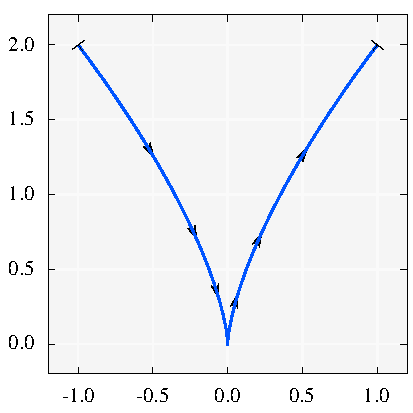
\includegraphics[width=\linewidth]{plots/curve-example-1.pdf}
      \caption{%
        Semicubical Parabola
        \[
          \begin{aligned}[t]
            &\function{γ}{[-1,1]}{\setReal^2} \\
            &γ(t) \define
            \begin{pmatrix}
              t^3 \\
              2t^2
            \end{pmatrix}
          \end{aligned}
        \]
      }
    \end{subfigure}
    \begin{subfigure}[t]{0.32\linewidth}
      \center
      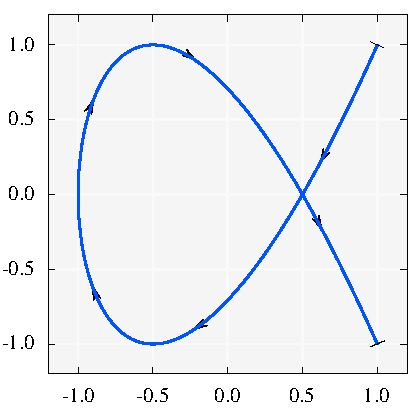
\includegraphics[width=\linewidth]{plots/curve-example-3.pdf}
      \caption{%
        Lissajous Curve
        \[
          \begin{aligned}[t]
            &\function{γ}{[0,2π]}{\setReal^2} \\
            &γ(t) \define
            \begin{pmatrix}
              \cos t \\
              \cos\roundBrackets{\frac{3}{2}t}
            \end{pmatrix}
          \end{aligned}
        \]
      }
    \end{subfigure}
    \begin{subfigure}[t]{0.32\linewidth}
      \center
      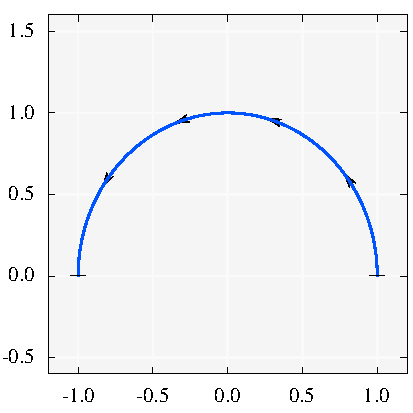
\includegraphics[width=\linewidth]{plots/curve-example-5.pdf}
      \caption{%
        Half-Circle
        \[
          \begin{aligned}[t]
            &\function{γ}{[0,π]}{\setReal^2} \\
            &γ(t) \define
            \begin{pmatrix}
              \cos t \\
              \sin t
            \end{pmatrix}
          \end{aligned}
        \]
      }
    \end{subfigure}

    \begin{subfigure}[t]{0.32\linewidth}
      \center
      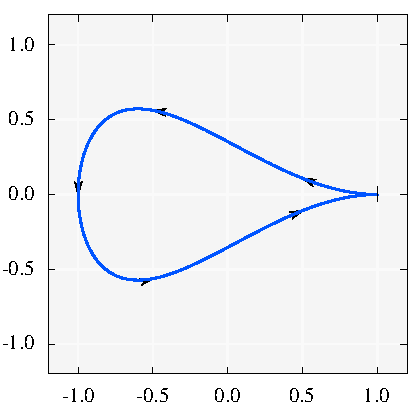
\includegraphics[width=\linewidth]{plots/curve-example-2.pdf}
      \caption{%
        Teardrop Curve
        \[
          \begin{aligned}[t]
            &\function{γ}{\mathds{T}^1[0,2π]}{\setReal^2}\\
            &γ(t) \define
            \begin{pmatrix}
              \cos(t) \\
              \sin(t)\sin^3\roundBrackets{\frac{1}{2}t}
            \end{pmatrix}
          \end{aligned}
        \]
      }
    \end{subfigure}
    \begin{subfigure}[t]{0.32\linewidth}
      \center
      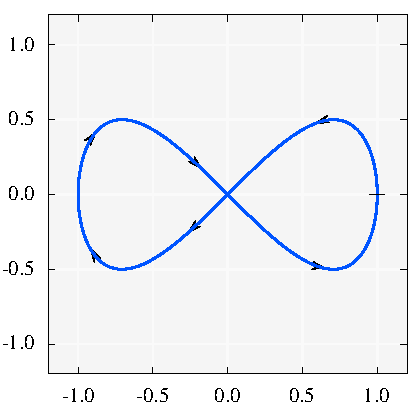
\includegraphics[width=\linewidth]{plots/curve-example-4.pdf}
      \caption{%
        Lissajous Curve
        \[
          \begin{aligned}[t]
            &\function{γ}{\mathds{T}^1[0,2π]}{\setReal^2} \\
            &γ(t)\define
            \begin{pmatrix}
              \cos t \\
              \frac{1}{2} \sin 2t
            \end{pmatrix}
          \end{aligned}
        \]
      }
    \end{subfigure}
    \begin{subfigure}[t]{0.32\linewidth}
      \center
      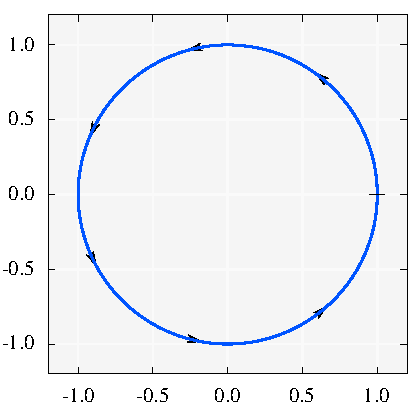
\includegraphics[width=\linewidth]{plots/curve-example-6.pdf}
      \caption{%
        Circle
        \[
          \begin{aligned}[t]
            &\function{γ}{\mathds{T}^1[0,2π]}{\setReal^2} \\
            &γ(t)\define
              \begin{pmatrix}
                \cos t \\
                \sin t
              \end{pmatrix}
          \end{aligned}
        \]
      }
    \end{subfigure}
    \caption[Examples of Smooth Parameterized Curves]{%
      \textbf{Examples of Smooth Parameterized Curves}\\
      All the plots show a smooth two-dimensional parameterized curve γ of a different class.
      The first row from left to right shows a general curve, a regular curve with self-intersection, and a regular and simple curve parameterized by arc length.
      The second row shows closed counterparts, respectively.
      Hereby, the black arrows indicate the orientation of the chosen parameterization and the black lines its start and end.
    }
    \label{fig:curve-examples}
  \end{figure}

  For most of the considered applications, the actual parameterization of a curve is not essential.
  Only the shape, given by its image, is used, referred, and transformed.
  But using only the shape and neglecting the parameterization of a curve does only make sense if the shape at least fulfills the properties of a one-dimensional manifold.
  Unfortunately, as can be seen in figure~\ref{fig:curve-examples}, the shape of parameterized curves may exhibit more general structures, such as sharp edges and self-intersections, and, thus, does not necessarily abide to these constraints.
  As a consequence, more regular and specialized classes of curves need to be looked at. \\
  \autocite{goldhorn2009,carmo2016,kuehnel2013}

  \begin{definition}[Regular and Simple Parameterized Curves]
    Let γ be a parameterized curve.
    Then γ is said to be simple if it is injective and regular if the following statement holds.
    \[
      \forall t\in \mathscr{D}(γ)^\circ \colon\quad γ'(t)\neq 0
    \]
    Furthermore, if $\norm{γ'} = 1$ then γ is parameterized by arc length.
  \end{definition}
  The definition states that the derivative of a regular curve is apart from its boundary never zero and therefore a map of full-rank at every inner point.
  Hence, a regular curve is an immersion into Euclidean space and, as a result, its shape is an immersed submanifold that still may contain self-intersections.
  Using a curve that is parameterized by arc length is hereby only a way of defining a canonical parameterization for regular curves that will be used to simplify the definition of curvature.
  It is clear by definition, that every curve parameterized by arc length is also a regular curve.
  \autocite{goldhorn2009,carmo2016,kuehnel2013}

  In applications that are able to handle self-intersections, regular curves are already sufficiently constrained.
  Indeed, a robust and stable algorithm for curve smoothing should be able to cope with self-intersections and even remove them if necessary.
  Still, to properly understand the transition, a regular curve shall become an embedding, such that, according to section~\ref{sec:analysis_on_manifolds}, its shape is actually a one-dimensional manifold.
  To state that a curve is also simple, ensures it exhibits no self-intersections other than the single intersection for closed curves.
  The results of the statements and thoughts of this and the previous paragraph are rigorously summarized in the following proposition.
  As this statement is a direct corollary, no additional rigorous proof will be given for it.
  % Then by application of the theorem, the image of the embedding is an embedded 1-manifold.
  \autocite{goldhorn2009,carmo2016,kuehnel2013}

  \begin{corollary}[Simple, Regular Curves are Embeddings]
    Let γ be a smooth parameterized curve that is simple and regular.
    Then γ is a smooth embedding into Euclidean space and its image is an orientable and connected one-dimensional submanifold with boundary.
    If γ is closed, then its image has no boundary.
  \end{corollary}
  The fundamental part of the concept of geodesics is the curvature.
  To gain an intuitive approach to a definition of curvature of a regular curve, we need to be able to evaluate its length and arc length in Euclidean space.
  These will allow us to properly provide a canonical parameterization to overall simplify the use of regular curves.

  \begin{definition}[Length of Curves]
    Let γ be a parameterized curve on $[a,b]$ or $\mathds{T}^1[a,b]$.
    Then the length $L(γ)$ and arc length, given by $\function{s_γ}{[a,b]}{[0,L(γ)]}$ or $\function{s_γ}{\mathds{T}^1[a,b]}{\mathds{T}^1[0,L(γ)]}$, respectively, of γ are defined by the following expressions.
    \[
      L(γ) \define \integral{a}{b}{\norm{γ'(t)}}{t}
      % \separate
      % \function{s_γ}{\mathscr{D}(γ)}{[0,L(γ)]}
      \separate
      s_γ(t) \define \integral{a}{t}{\norm{γ'(x)}}{x}
    \]
  \end{definition}
  The definition of the length and arc length mainly stems from the physical interpretation that a parameterized curve is a trajectory in space over time of a particle moving with a specific velocity that is given by the derivative of the curve's parameterization.
  For evaluating the distance covered, one needs to integrate over the speed, that is given by the magnitude of the velocity, at each point in time.

  For every parameterized curve γ, the length and arc length are well-defined because the function $\norm{γ'}$ is continuous on a compact set and, consequently, uniformly continuous.
  Hence, the integral expressions defining $L(γ)$ and $s_γ$ are finite and well-behaved.
  Furthermore, according to the fundamental theorem of calculus \autocite{forster2016,elstrodt2011}, $s_γ$ is continuously differentiable with derivative $s_γ' = \norm{γ'}$ and surjective.
  A direct consequence for curves parameterized by arc length is that their length can be simply computed by $L(γ)=b-a$.
  This simplification leads to the idea to reparameterize general regular curves, such that they become curves parameterized by arc length and, accordingly, inheriting their good properties.
  The details for this approach are given by the following lemma for open parameterized curves as closed curves can be seen as a special kind of open curve.

  \begin{lemma}[Regular curves can be parameterized by arc length]
    Let $n\in\setNatural$, $k\in\setNatural_{\infty}$, $[a,b]\subset\setReal$ be a compact interval, and $\function{γ}{[a,b]}{\setReal^n}$ be an $n$-dimensional parameterized curve of class $\mathrm{C}^k$ that is regular.
    Then up to a constant shift, there exists a unique $k$-times continuously differentiable and bijective function $\function{u}{[c,d]}{[a,b]}$ on a compact interval $[c,d]\subset\setReal$ with strictly positive derivative, such that the composition $γ\composition u$ is a curve parameterized by arc length.
  \end{lemma}
  \begin{proof}
    The restriction of $\norm{\cdot}$ to $\setReal^n\setminus\set{0}{}$ is an infinitely differentiable function.
    The regularity of γ implies that $\norm{γ'}$ and, as a direct consequence, the derivative of $s_γ$ are strictly positive on $(a,b)$.
    Hence, $s_γ$ is bijective with $k$-times continuously differentiable inverse.
    The derivative of $s_γ^{-1}$ must also be strictly positive in the interior and continuous as a composition of continuous functions.
    \[
      \roundBrackets{s_γ^{-1}}' = \frac{1}{s_γ'\composition s_γ^{-1}} = \frac{1}{\norm{γ'}\composition s_γ^{-1}} > 0
    \]
    Define $\tilde{γ}\define γ\composition s_γ^{-1}$.
    Then by differential calculus, it follows, that $\tilde{γ}$ is $k$-times continuously differentiable and parameterized by arc length.
    \[
      \norm{\tilde{γ}'}
      = \norm{γ'\composition s_γ^{-1} \cdot \roundBrackets{s_γ^{-1}}'}
      = \norm{\frac{γ'\composition s_γ^{-1}}{s_γ'\composition s_γ^{-1}}}
      = \norm{\frac{γ'\composition s_γ^{-1}}{\norm{γ'}\composition s_γ^{-1}}}
      = \frac{\norm{γ'\composition s_γ^{-1}}}{\norm{γ'\composition s_γ^{-1}}}
      = 1
    \]
    This shows that $s_γ^{-1}$ fulfills the required properties and the existence of a parameterization by arc length.
    To show its uniqueness up to a constant shift, assume an arbitrary function $u$ as given in the lemma.
    Applying the same reasoning as for $s_γ$, it is clear that $\inverse{u}$ also is $k$-times continuously differentiable with strictly positive derivative on the interior.
    By calculation, we may then show its connection to the arc length.
    \[
      1
      = \norm{(γ\composition u)'}
      = \norm{γ'\composition u} \cdot u'
      = \frac{\norm{γ'\composition u}}{\roundBrackets{\inverse{u}}'\composition u}
      = \frac{\norm{γ'}}{\roundBrackets{\inverse{u}}'}
      \quad\implies\quad
      \norm{γ'} = \roundBrackets{\inverse{u}}'
    \]
    To integrate this formula, let $t\in[a,b]$ be arbitrary and use again the fundamental theorem of calculus.
    \[
      s_γ(t)
      = \integral{a}{t}{\norm{γ'(x)}}{x}
      = \integral{a}{t}{\roundBrackets{\inverse{u}}'(x)}{x}
      = \inverse{u}(t) - \inverse{u}(a)
      = \inverse{u}(t) - c
    \]
    \[
      u = s_γ^{-1}\composition s_γ\composition u
      = s_γ^{-1}(\cdot - c)\composition \inverse{u}\composition u
      = s_γ^{-1}\roundBrackets{\cdot - c}
    \]
    This shows that, up to a constant shift, $u$ is the same as $s_γ^{-1}$ and the uniqueness of the parameterization by arc length.
  \end{proof}
  The proof above shows, that the inverse of the arc length of a regular curve up to some shifting can be used as a unique reparameterization to transform it into a curve parameterized by arc length.
  In this sense, the lemma makes clear that it is sufficient to handle curves that are parameterized by arc length instead of general regular curves.
  According to this, we will define this as the canonical parameterization of a regular curve.

  \begin{definition}[Canonical Parameterization by Arc Length]
    Let γ be a regular curve.
    Then its canonical parameterization by arc length $\bar{γ}$ is defined by the following expression.
    \[
      \bar{γ} \define γ\composition s_γ^{-1}
    \]
  \end{definition}
  For smooth curves parameterized by arc length, the definition of their curvature is now straight-forward, as we understand it as the amount the curve bends at a point when moving along its trajectory.
  Referring to differential calculus, the magnitude of the second derivative exactly describes this specific amount.

  \begin{definition}[Curvature of Regular Curves]
    Let $k\in\setNatural_\infty$ with $k\geq 2$, γ be a curve parameterized by arc length of class $\mathrm{C}^k$, and φ be a regular curve of class $\mathrm{C}^k$.
    Their respective curvatures $κ(γ)$ and $κ(φ)$ are defined by the following expressions.
    \[
      κ(γ)\define\norm{γ''}
      \separate
      κ(φ)\define κ(\bar{φ})\composition s_φ
    \]
  \end{definition}
  The definition involves second-order derivatives and therefore at least requires the curves to be of class $\mathrm{C}^2$.
  In differential geometry, only smooth curves are typically observed where this states no further constraints.
  For general regular curves, the tangent vector is not normalized which results in a scaling of the curvature value.
  The definition omits this peculiarity by using the arc length function to get back to the original parameterization.

  To finally provide a definition for geodesics, it is no longer sufficient to look at smooth curves freely traversing the Euclidean space.
  Instead, we will embed curves into smooth surfaces which already exhibit intrinsic curvature.
  Based on this intrinsic curvature, the overall curvature of a curve can be decomposed into the geodesic and normal curvature.
  Hereby, the geodesic curvature describes the amount of curvature an intrinsic observer of the ambient surface would measure walking along the curve without knowledge of the extrinsic curvature.
  The normal curvature on the other hand is only observable from the ambient space and depends on the extrinsic curvature and the tangential vector of the curve.
  In the context of curve smoothing, the surfaces, we are looking at, are given by compact (orientable) Riemannian submanifolds (with boundary) of dimension two embedded in $\setReal^3$.

  \begin{definition}[Geodesic and Normal Curvature of Curves]
    Let $M$ be a Riemannian submanifold embedded in $\setReal^n$ and γ be a curve parameterized by arc length and embedded in $M$.
    The geodesic curvature $κ_\mathrm{g}(M,γ)$ and the normal curvature $κ_\mathrm{n}(M,γ)$ are given by the following expressions.
    \[
      κ_\mathrm{g}(M,γ) \define \norm{P_{\mathrm{T}_{γ}M} (γ'')}
      \separate
      κ_\mathrm{n}(M,γ) \define \norm{P_{\mathrm{N}_{γ}M} (γ'')}
    \]
  \end{definition}
  Geodesic and normal curvature are simply defined by computing the norm of projecting the direction of bending into the tangential and normal space of the manifold, respectively.
  Hence, this definition is consistent with the interpretation given above.
  As a direct consequence of the definition, the following statement can be deduced without further proof.

  \begin{corollary}
    Let $M$ be a Riemannian submanifold embedded in $\setReal^n$ and γ be a curve embedded in $M$  and parameterized by arc length.
    \[
      κ^2(γ) = κ_\mathrm{g}^2(M,γ) + κ_\mathrm{n}^2(M,γ)
    \]
  \end{corollary}
  This statement may also be used to generalize the normal curvature for polyhedral surfaces.

  Up to now, all curvature definitions have been non-negative scalar functions that did not provide any orientation.
  But in the context of orientable Riemannian submanifolds of dimension two, further knowledge about the direction of geodesic bending can be provided.
  This is especially useful for implementation-specific work.
  Providing orientations for manifolds and curves allows for a more efficient moving of points along a curve or surface and access to its neighbors.

  \begin{definition}[Oriented Curvatures of Curves]
    Let $M$ be a two-dimensional oriented Riemannian submanifold embedded in $\setReal^3$ and γ a curve embedded in $M$ parameterized by arc length.
    Let $\function{ν}{M}{\mathrm{N}M}$ be a field of positively oriented unit normals on $M$ and $\function{μ}{M}{\mathrm{T}M}$ be a field of tangent vectors such that $(γ',μ\circ γ)$ is positively oriented basis.
    \[
      κ_\mathrm{g}(M,γ) = \scalarProduct{μ\circ γ}{γ''}
      \separate
      κ_\mathrm{n}(M,γ) = \scalarProduct{ν\circ γ}{γ''}
    \]
  \end{definition}

  \begin{definition}[Geodesics]
    Let $M$ be a two-dimensional Riemannian submanifold embedded in $\setReal^3$ and $\function{γ}{[a,b]}{M}$ a curve parameterized by arc length.
    The curve γ is called a geodesic if $κ_g(γ) = 0$.
  \end{definition}

  \begin{definition}[Geodesics Problems]
    Let $M$ be a two-dimensional Riemannian submanifold embedded in $\setReal^3$.

    The problem of finding a geodesic $\function{γ}{[a,b]}{M}$ for a given starting point $γ(a)$ and a given direction $γ'(a)$ is called the geodesic initial value problem.

    The problem of finding a geodesic $\function{γ}{[a,b]}{M}$ for given start and end points $γ(a)$ and $γ(b)$ is called the geodesic boundary value problem.
  \end{definition}

% subsection differential_geometry (end)

\subsection{Polyhedral Surfaces} % (fold)
\label{sub:polyhedral_surfaces}

  There are definitions for manifolds with corners.
  In the topological case, these are equivalent to manifolds with boundaries.
  For the smooth case, it is different.
  The half space is only homeomorphic and not diffeomorphic to the cube space.
  so, we could generalize a polyhedral surface as a smooth manifold with corners.
  on the definitions, there is no uniform agree.
  So, we will not use the generalization of manifolds with corners.
  we will use the theory of polthier which should be applicable to manifolds with corners.

  \begin{definition}[Triangle]
    Let $n\in\setNatural$ with $n\geq 2$ and $A,B,C\in\setReal^n$ affinely independent points.
    Then the (topological) triangle $\triangle$ (embedded in $\setReal^n$) is given by the following expression.
    \[
      \triangle \define \set{uA + vB + wC}{u,v,w\in[0,1], u+v+w=1}
    \]
    The triangle's vertices $\mathscr{V}(\triangle)$ and edges $\mathscr{E}(\triangle)$ are hereby defined as follows.
    \[
      \mathscr{V}(\triangle) \define \set{A,B,C}{}
      \separate
      \mathscr{E}(\triangle) \define \set{\overline{AB}, \overline{BC}, \overline{CA}}{}
    \]
    \[
      \partial\triangle \define \textstyle\bigcup\mathscr{E}(\triangle)
    \]
    \[
      Π \define \set{\function{π}{\set{1,2,3}{}}{\mathscr{V}(\triangle)}}{\text{π bijective}}
    \]
    \[
      D \define \set{(u,v) \in [0,1]^2}{u + v < 1}
    \]
    \[
      \function{φ_π}{\overline{D}}{\triangle}
      \separate
      φ_π(u,v) \define (1 - u - v) π(1) + u π(2) + v π(3)
    \]
    \[
      π\sim π' :\iff \exists σ\in\mathrm{S}_3, \mathrm{sgn}\, σ = 1 \colon π' = π\circ σ
    \]
    \[
      Π/\sim = \set{[π], [\bar{π}]}{}
    \]
    \[
      \triangle_{[π]} \define (\triangle, [π])
    \]
    \[
      \mathscr{E}(\triangle_{[π]}) \define \set{\overrightarrow{π_1π_2},\overrightarrow{π_2π_3}, \overrightarrow{π_3π_1}}{}
    \]
    \[
      ϑ_\triangle(A) = \arccos\frac{\scalarProduct{\overrightarrow{AB}}{\overrightarrow{AC}}}{\norm{\overrightarrow{AB}}\norm{\overrightarrow{AC}}}
    \]
  \end{definition}
  A triangle is an orientable topological 2-manifold with boundary embedded in $\setReal^n$.
  The atlas is given by $\set{\roundBrackets{φ_π(D),φ_π|_D^{-1}}}{π\in Π}$
  The inner set $\triangle^\circ$ is an orientable smooth 2-manifold without boundary.
  Its atlas is given by the restrictions $(\triangle^\circ, φ_π|_{D^\circ}^{-1})$.
  Triangles are planar surfaces and, hence, geodesics are given by straight lines.
  Furthermore, the triangle is by definition a convex set and therefore always provides a unique solution for the geodesic boundary value problem.

  \begin{definition}[Polyhedral Surface and Surface Mesh]
    Let $n\in\setNatural$ with $n\geq 2$ and $\mathscr{T}\neq\emptyset$ be a finite set of triangles embedded in $\setReal^n$.
    Let $S=\bigcup\mathscr{T}$ be a two-dimensional topological manifold (with boundary), such that for all $\triangle_1,\triangle_2\in\mathscr{T}$ with $\triangle_1\neq\triangle_2$ the following holds.
    \[
      \triangle_1\cap\triangle_2 \in \set{\emptyset}{} \cup [\mathscr{V}(\triangle_1)\cap\mathscr{V}(\triangle_2)] \cup [\mathscr{E}(\triangle_1)\cap\mathscr{E}(\triangle_2)]
    \]
    In this case, $S$ is called a (topological) polyhedral surface (embedded in $\setReal^n$).
    With $\mathscr{V}(S)$ we denote its vertices, with $\mathscr{E}(S)$ its edges, and with $\mathscr{F}(S)$ its faces.
    \[
      \mathscr{V}(S) \define \bigcup_{\triangle\in\mathscr{T}} \mathscr{V}(\triangle)
      \separate
      \mathscr{E}(S) \define \bigcup_{\triangle\in\mathscr{T}} \mathscr{E}(\triangle)
      \separate
      \mathscr{F}(S) \define \mathscr{T}
    \]
    (topological) surface mesh.
    \[
      \mathscr{M}(S) \define \textstyle\bigcup \mathscr{E}(S)
    \]
    \[
      \partial\mathscr{E}(S) \define \set{e\in\mathscr{E}(S)}{\exists!\triangle\in\mathscr{F}(S)\colon e\subset\triangle}
      \separate
      \mathscr{E}^\circ(S) \define \mathscr{E}(S) \setminus \partial\mathscr{E}(S)
    \]
    \[
      \partial S \define \textstyle\bigcup \partial\mathscr{E}(S)
      \separate
      \partial\mathscr{V}(S) \define \mathscr{V}(S) \cap \partial S
      \separate
      \mathscr{V}^\circ(S) \define \mathscr{V}(S) \setminus \partial\mathscr{V}(S)
    \]
  \end{definition}
  A surface mesh is again a topological 2-manifold.

  \begin{definition}[Oriented Surface Mesh]
    Let $S$ be a surface mesh and $\function{Π}{\mathscr{F}(S)}{\bigsqcup_{\triangle\in\mathscr{F}(S)} Π_\triangle}$.
    \[
      \forall \triangle_1,\triangle_2\in\mathscr{F}(S),\triangle_1\neq\triangle_2\colon\quad \mathscr{E}(Π(\triangle_1)) \cap \mathscr{E}(Π(\triangle_2)) = \emptyset
    \]
    $(S,Π)$ is called an oriented surface mesh.
  \end{definition}

  \begin{definition}[Discrete Surface Mesh Curve]
    Let $n\in\setNatural$, $S$ be a surface mesh, and $x\in \boxBrackets{\bigcup\mathscr{E}(S)}^{n+1}$ be a tuple of $n+1$ points on the edges of the surface mesh $S$, such that adjacent points lie on the same triangle.
    \[
      \forall k\in\setNatural,k\leq n\colon x_k\neq x_{k+1} \land \exists \triangle\in\mathscr{F}(S)\colon x_k, x_{k+1}\in\triangle
    \]
    The (topological) curve given by connecting adjacent points by a straight line is called the (topological) discrete surface mesh curve.
  \end{definition}

  \begin{definition}[Surface Mesh Curve without Artifacts]
    Let $S$ be a polyhedral surface and γ be a surface mesh curve characterized by $x\in\mathscr{M}^{n+1}(S)$.
    \[
      \forall k\in\setNatural, 1\leq k \leq n\colon
      \mathscr{F}_S(x_{k-1}) \cap \mathscr{F}_S(x_{k+1}) = \emptyset
    \]
    If γ is a closed curve, that is $x_0 = x_{n+1}$, then
    \[
      \mathscr{F}_S(x_1) \cap \mathscr{F}_S(x_n) = \emptyset
    \]
  \end{definition}

  \begin{definition}[Total Vertex Angle]
    \[
      ϑ_S(v) \define \sum_{\triangle\in\mathscr{T}, v\in\triangle} ϑ_\triangle(v)
    \]
  \end{definition}

  \begin{definition}[Curve Angle]
    Let $S$ be a polyhedral surface and $p,x,q\in\mathscr{M}(S)$, $x\in S^\circ$ be adjacent vertices of surface mesh curve without artifacts on $S$.
    Let $\mathscr{V}_S(x)$ the neighboring vertices.
    The neighbor set can be partitioned into three possible empty tuples, such that $p,(x),q$ is surface mesh curvature without artifacts.
    There exists two tuples $(p=x_{λ(0)},x_{λ(1)},\ldots,x_{λ(n)},x_{λ(n+1)} = q)$ and $(p,x_{ρ(1)},\ldots,x_{ρ(m)},q)$ that characterize a surface mesh curve without artifacts.
    \[
      β_λ = \sum_{k=1}^n \sphericalangle(x_{λ(k-1)},x_{λ(k)},x_{λ(k+1)})
      \separate
      β_ρ = \sum_{k=1}^m \sphericalangle(x_{ρ(k-1)},x_{ρ(k)},x_{ρ(k+1)})
    \]
    The (unoriented) curve angle at $x$ is given by the sum
    \[
      β = \min \set{β_λ, β_ρ}{}
    \]
    If there is an orientation $Π$ for $S$ then the (oriented) curve angle is given by the segmentation which points are connected by directed edge paths in their respective triangles such that $x$ is not contained.
  \end{definition}
  For the oriented case, the curve angle can only be defined for curve vertices that do not lie on the boundary of $S$.
  Also the interpretation of the total vertex angle for boundary points is different.
  This makes a generalization of the oriented discrete curvature at boundary points difficult.

  \begin{definition}[Discrete Geodesic Curvature]
    \[
      κ_\mathrm{g}(γ) = π - \frac{2π}{ϑ_S(γ)}β_S(γ)
    \]
  \end{definition}

  \begin{definition}[Discrete Geodesic Curvature for Boundaries]

  \end{definition}

  \begin{definition}[Discrete Geodesic Problems]

  \end{definition}

% subsection polyhedral_surfaces (end)

% Differential Geometry on Polyhedral Surfaces
% \autocite{polthier2006}

% Curvature Estimation on Surfaces
% \autocite{rusinkiewicz2004}

% Generation of Surface Normals
% \autocite{max1999,meyer2001,jin2005}

% section preliminaries (end)
\end{document}
